\documentclass[border=4pt]{standalone}
\usepackage{tikz}
\usetikzlibrary{arrows.meta,shapes.multipart}
\begin{document}
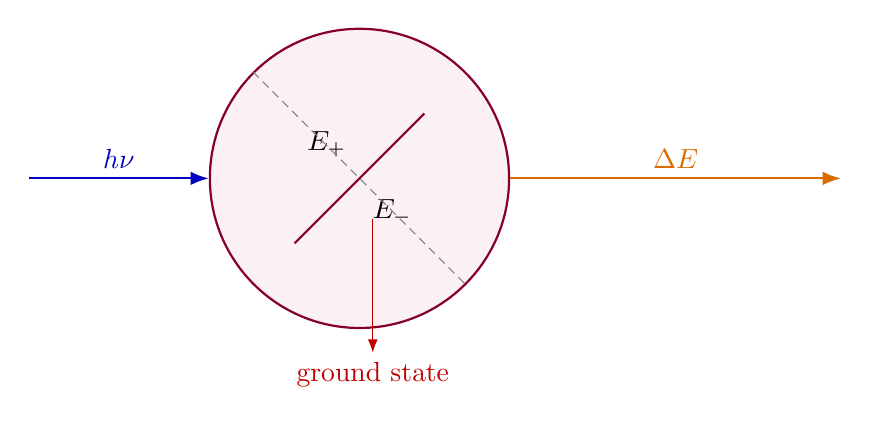
\begin{tikzpicture}[>=Latex]
  \node[circle solidus,draw=purple!70!black,thick,fill=purple!6,
    inner xsep=7pt,inner ysep=5pt,minimum size=38mm] (levels)
    {$E_+$\nodepart{lower}$E_-$};

  \draw[-Latex,thick,blue!75!black] (-42mm,0) --
    node[above] {$h\nu$} (levels.west);
  \draw[-Latex,thick,orange!85!black] (levels.east) --
    node[above] {$\Delta E$} ++(42mm,0);
  \draw[-Latex,red!75!black] (levels.lower) -- ++(0,-17mm)
    node[below] {ground state};
  \draw[gray,densely dashed] (levels.north west) --
    (levels.south east);
\end{tikzpicture}
\end{document}
